\documentclass[english,3p]{elsarticle}

\usepackage[T1]{fontenc}
\usepackage[utf8]{inputenc}
\usepackage{babel}
\usepackage{color}
\usepackage[usenames,dvipsnames]{xcolor}
\usepackage{bm}
\usepackage{setspace}
\usepackage{amssymb}
\usepackage{amsmath}
\usepackage{amsfonts}

\newcommand{\todo}[1]{\colorbox{yellow}{\textbf{#1}}}
\newcommand{\code}[1]{\texttt{#1}}
\newcommand{\ii}{\mathrm{i}}
\newcommand{\ee}{\mathrm{e}}
\newcommand{\dd}{\mathrm{d}}

\usepackage{listings}
\usepackage{color}

\definecolor{mygreen}{rgb}{0,0.6,0}
\definecolor{mygray}{rgb}{0.5,0.5,0.5}
\definecolor{mymauve}{rgb}{0.58,0,0.82}

\lstdefinestyle{customc}{
  belowcaptionskip=1\baselineskip,
  breaklines=true,
  frame=l,
  xleftmargin=\parindent,
  language=C,
  showstringspaces=false,
  basicstyle=\footnotesize\ttfamily,
  keywordstyle=\bfseries\color{green!40!black},
  commentstyle=\itshape\color{purple!40!black},
  identifierstyle=\color{blue},
  stringstyle=\color{orange},
}
\lstdefinestyle{customasm}{
  belowcaptionskip=1\baselineskip,
  frame=L,
  xleftmargin=\parindent,
  language=[x86masm]Assembler,
  basicstyle=\footnotesize\ttfamily,
  commentstyle=\itshape\color{purple!40!black},
}
\lstset{escapechar=@,style=customc}

\begin{document}

\begin{center}
\textbf{EAA Winter School in Computational Acoustics}

Tutorial on FreeFEM++
\end{center}

\vspace{10mm}

This part of the tutorial on finite elements uses the FreeFEM++ package which is freely available at ???.
It is already installed on the workstations.
To use it you can...

\section{Sound field in a cavity}

We begin with the calculation of the sound field in a cavity with a vibrating wall.
The first part of the file \code{cavity.edp} defines a number of boundaries for the computational domain and plot the resulting geometry (using 20 points per boundary):
\begin{lstlisting}
// Create the boundaries of the computational domain
border a0(t=0,1) { x= 5; y= 1+2*t ;}
border a1(t=0,1) { x=5-2*t; y= 3 ;} 
border a2(t=0,1) { x= 3-2*t; y=3-2*t ;}
border a3(t=0,1) { x= 1-t; y= 1 ;} 
border a4(t=0,1) { x= 0; y= 1-t ;} 
border a5(t=0,1) { x= t; y= 0 ;} 
border a6(t=0,1) { x= 1+4*t; y= t ;}

// Plot the geometry of the computational domain
plot( a0(20) + a1(20)+ a2(20) +  a3(20) + a4(20) + a5(20) + a6(20),wait=1,ps="domain.eps" );
\end{lstlisting}
This results in figure \ref{fig:geometry}
\begin{figure}[h]
\centering
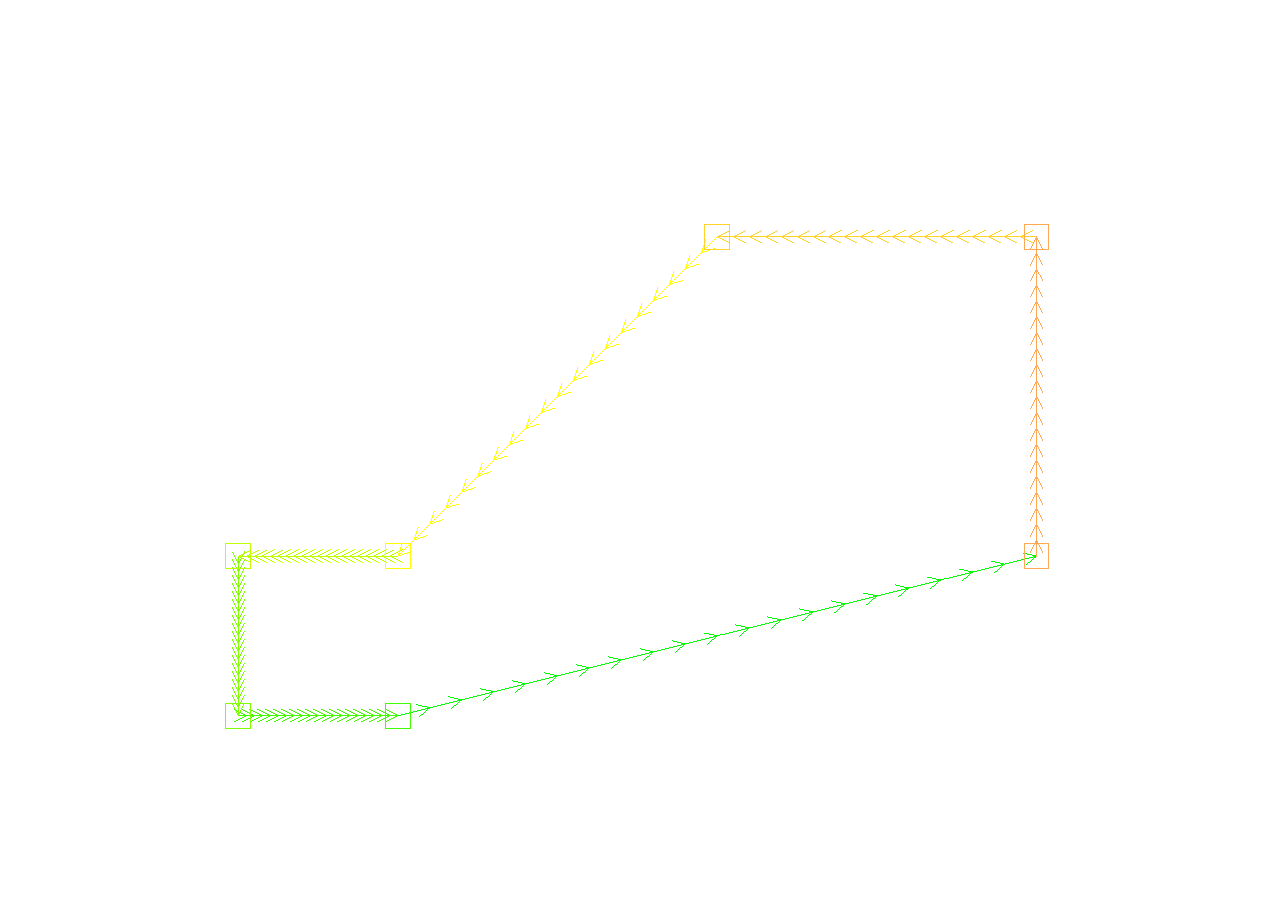
\includegraphics[width=80mm]{domain.eps}
\caption{Geometry of the computational domain}
\label{fig:geometry}
\end{figure}

The next step is to generate a mesh of the computational domain using triangular elements:
\begin{lstlisting}
// Generate a mesh of the domain using 20 elements per edge
mesh Th=buildmesh( a0(20) + a1(20)+ a2(20) +  a3(20) + a4(20) + a5(20) + a6(20) );
\end{lstlisting}
The mesh can then be shown using the following command, resulting in figure
\begin{lstlisting}
// Plot the mesh
plot(Th, wait=1, ps="Th.eps");
\end{lstlisting}
\begin{figure}[h]
\centering
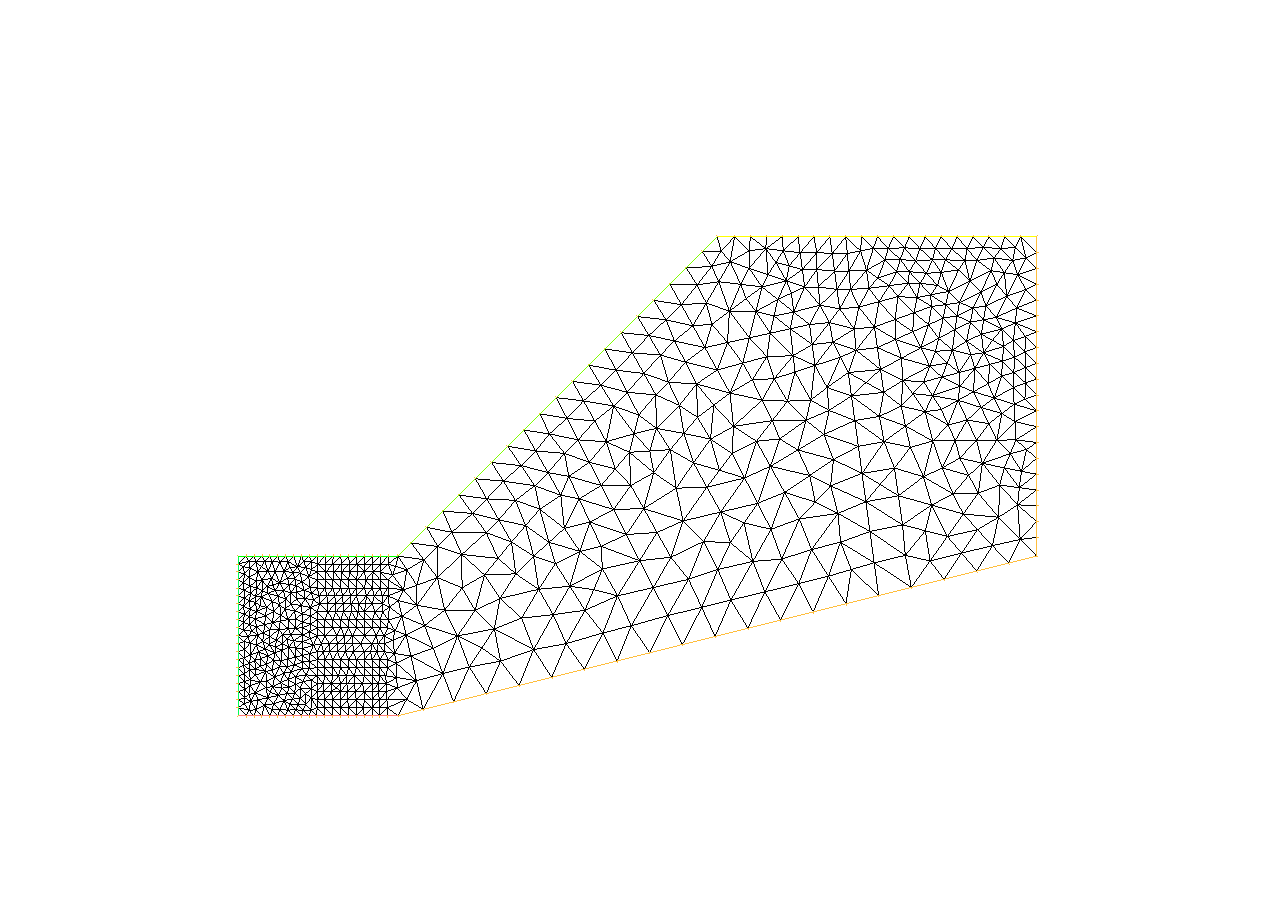
\includegraphics[width=80mm]{mesh.eps}
\caption{Mesh of the computational domain}
\label{fig:mesh}
\end{figure}

We define the approximation space which is formed of linear interpolation functions on the mesh previously created:
\begin{lstlisting}
// Define the approximation space based on linear elements
fespace Vh(Th,P1);
Vh p,q;
\end{lstlisting}

Finally we can solve the variational formulation for the Helmholtz equation
$$
\int_\Omega k^2qp - \nabla q\cdot\nabla p\,\dd\Omega+
\int_{\Gamma_4} q\,\dd\Gamma
=0
\;.
$$
\begin{lstlisting}
// Solve the variational formulation for the Helmholtz equation
real k = 10;
solve cavity(p,q)=int2d(Th)(k*k*p*q - dx(p)*dx(q) - dy(p)*dy(q)) - int1d(Th,a4)(q);
\end{lstlisting}
In this code we have set $k=10$.

We can plot the pressure field given by the finite-element model:
\begin{lstlisting}
// Plot the result
plot(p, fill=1);
\end{lstlisting}
which gives figure \ref{fig:solution1}.
\begin{figure}[h]
\centering
\includegraphics[width=80mm]{solution1.eps}
\caption{Solution of the cavity problem using linear elements and 20 elements per boundary.}
\label{fig:solution1}
\end{figure}

\textbf{Question 1:} Switch to a quadratic approximation space by using \code{P2} instead of \code{P1} in the definition of the approximation spaces \code{p} and \code{q}.

\textbf{Question 2:} Using a linear approximation of the solution, use a finer mesh with 40 element along each boundary.
For $k=10$, how many elements per wavelength does this correspond to?

\textbf{Question 3:} Of the two solutions produced in the previous two questions which one appears the more accurate? Why?

\textbf{Question 4:} Change the variational formulation in the file \code{cavity.edp} so that the forcing is applied on the boundary $\Gamma_6$.

\section{Vibration of a tuning fork}

The second example we consider is the modes of vibration of a tuning fork in two dimensions.
The input file for FreeFEM++ is called \code{tuning\_fork.edp}.
Please read through the comments included in this file.
The vibration of the tuning fork follows the equation of linear elasticity in the time-harmonic regime:
$$
-\omega^2\mathbf{u} = \nabla\cdot\boldsymbol{\sigma}
\;,\quad
\boldsymbol{\sigma} = \lambda\nabla\cdot\mathbf{u} + 2\mu\boldsymbol{\varepsilon}
$$
where $\mathbf{u}$ is the displacement of the elastic solid.
$\boldsymbol{\varepsilon}$ is the strain tensor and $\lambda$ and $\mu$ are the Lamé constant.
After generating a mesh of the tuning fork, the script calculates the mass and stiffness matrices.
An eigenvalue problem is then solved to find the resonance frequencies $\omega$ of the tuning fork as well as the associated displacement fields.

\textbf{Question 5:} Increase the mesh resolution and see how this influences the resonance frequencies.

\end{document}
